\documentclass{standalone}
\usepackage{tikz}
\usetikzlibrary{patterns, positioning}


\begin{document}
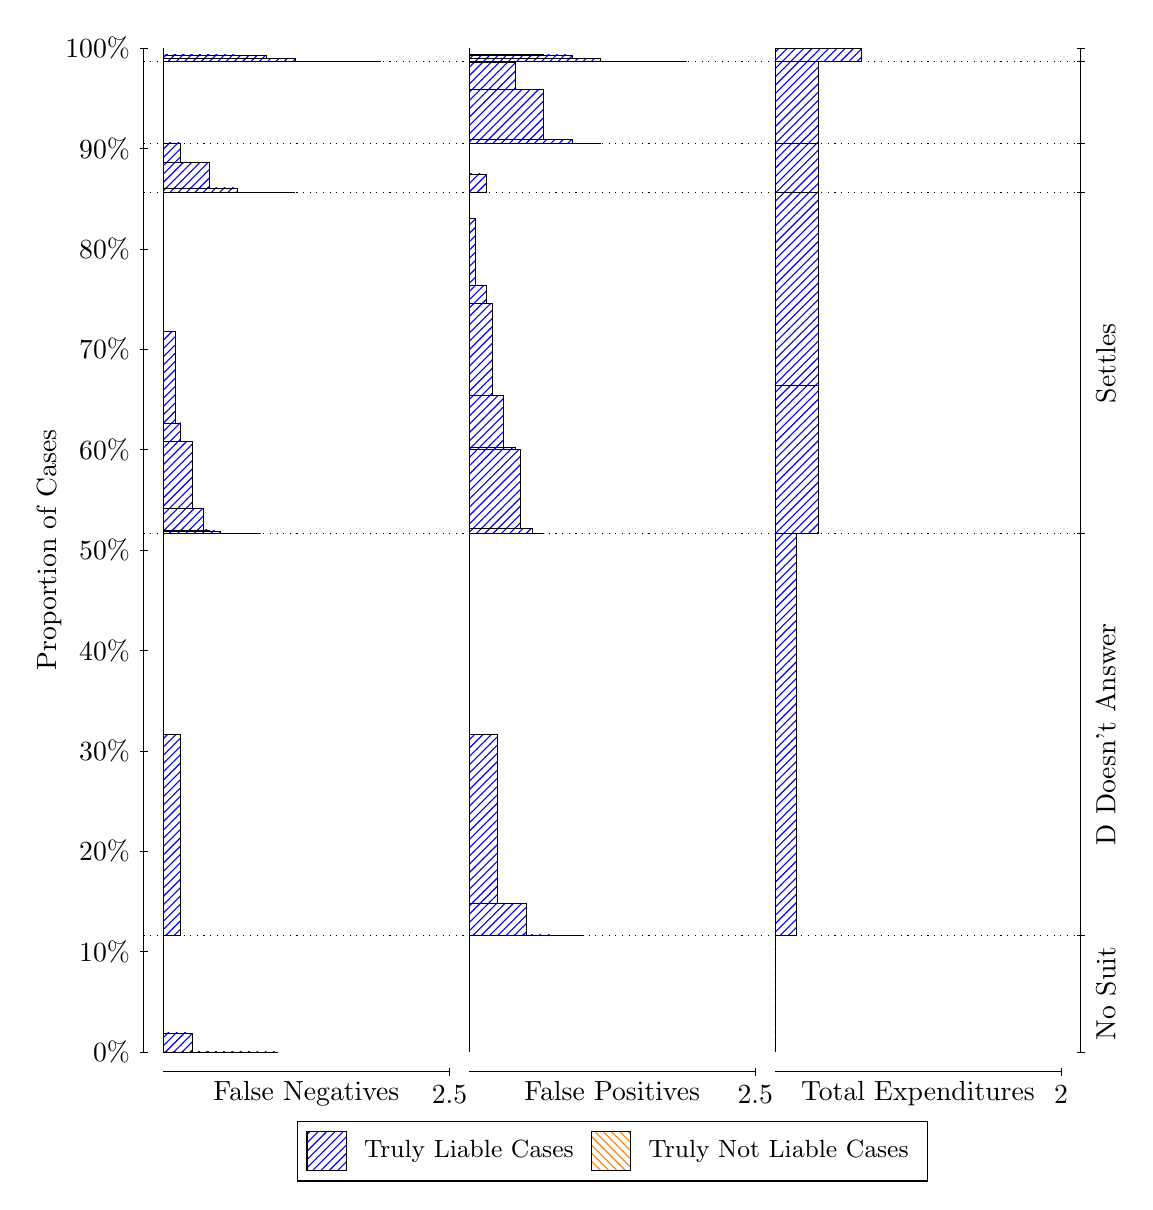
\begin{tikzpicture}
\draw[black, very thin] (1.5,1.75) -- (1.5,14.5);
\node[rotate=90, text=black, anchor=center] at (0.3, 8.125) {Proportion of Cases};
\draw[black, very thin] (1.45,1.75) -- (1.55,1.75);
\node[text=black, anchor=east] at (1.45, 1.75) {0\%};
\draw[black, very thin] (1.45,3.025) -- (1.55,3.025);
\node[text=black, anchor=east] at (1.45, 3.025) {10\%};
\draw[black, very thin] (1.45,4.3) -- (1.55,4.3);
\node[text=black, anchor=east] at (1.45, 4.3) {20\%};
\draw[black, very thin] (1.45,5.575) -- (1.55,5.575);
\node[text=black, anchor=east] at (1.45, 5.575) {30\%};
\draw[black, very thin] (1.45,6.85) -- (1.55,6.85);
\node[text=black, anchor=east] at (1.45, 6.85) {40\%};
\draw[black, very thin] (1.45,8.125) -- (1.55,8.125);
\node[text=black, anchor=east] at (1.45, 8.125) {50\%};
\draw[black, very thin] (1.45,9.4) -- (1.55,9.4);
\node[text=black, anchor=east] at (1.45, 9.4) {60\%};
\draw[black, very thin] (1.45,10.675) -- (1.55,10.675);
\node[text=black, anchor=east] at (1.45, 10.675) {70\%};
\draw[black, very thin] (1.45,11.95) -- (1.55,11.95);
\node[text=black, anchor=east] at (1.45, 11.95) {80\%};
\draw[black, very thin] (1.45,13.225) -- (1.55,13.225);
\node[text=black, anchor=east] at (1.45, 13.225) {90\%};
\draw[black, very thin] (1.45,14.5) -- (1.55,14.5);
\node[text=black, anchor=east] at (1.45, 14.5) {100\%};

\draw[black, very thin] (13.4,1.75) -- (13.4,14.5);
\draw[black, very thin] (13.35,1.75) -- (13.45,1.75);
\node[anchor=west] at (13.35, 1.75) {};
\draw[black, very thin] (13.35,3.2346) -- (13.45,3.2346);
\node[anchor=west] at (13.35, 3.2346) {};
\draw[black, very thin] (13.35,8.3327) -- (13.45,8.3327);
\node[anchor=west] at (13.35, 8.3327) {};
\draw[black, very thin] (13.35,12.662) -- (13.45,12.662);
\node[anchor=west] at (13.35, 12.662) {};
\draw[black, very thin] (13.35,13.29) -- (13.45,13.29);
\node[anchor=west] at (13.35, 13.29) {};
\draw[black, very thin] (13.35,14.329) -- (13.45,14.329);
\node[anchor=west] at (13.35, 14.329) {};
\draw[black, very thin] (13.35,14.5) -- (13.45,14.5);
\node[anchor=west] at (13.35, 14.5) {};

\draw[black, very thin, pattern color=blue, pattern=north east lines] (1.75,1.75) rectangle (3.2033,1.75);
\draw[black, very thin, pattern color=blue, pattern=north east lines] (1.75,1.75) rectangle (2.84,1.75);
\draw[black, very thin, pattern color=blue, pattern=north east lines] (1.75,1.75) rectangle (2.4767,1.7521);
\draw[black, very thin, pattern color=blue, pattern=north east lines] (1.75,1.7521) rectangle (2.1133,1.9931);
\draw[black, very thin, pattern color=orange, pattern=north west lines] (1.75,1.9931) rectangle (1.75,1.9931);
\draw[black, very thin, pattern color=blue, pattern=north east lines] (1.75,1.9931) rectangle (1.75,3.2346);
\draw[black, very thin, pattern color=blue, pattern=north east lines] (1.75,3.2346) rectangle (1.968,5.7804);
\draw[black, very thin, pattern color=orange, pattern=north west lines] (1.75,5.7804) rectangle (1.75,5.7804);
\draw[black, very thin, pattern color=blue, pattern=north east lines] (1.75,5.7804) rectangle (1.75,8.3327);
\draw[black, very thin, pattern color=blue, pattern=north east lines] (1.75,8.3327) rectangle (2.9853,8.3327);
\draw[black, very thin, pattern color=blue, pattern=north east lines] (1.75,8.3327) rectangle (2.84,8.3327);
\draw[black, very thin, pattern color=blue, pattern=north east lines] (1.75,8.3327) rectangle (2.6947,8.3327);
\draw[black, very thin, pattern color=blue, pattern=north east lines] (1.75,8.3327) rectangle (2.622,8.3381);
\draw[black, very thin, pattern color=blue, pattern=north east lines] (1.75,8.3381) rectangle (2.4767,8.3683);
\draw[black, very thin, pattern color=blue, pattern=north east lines] (1.75,8.3683) rectangle (2.3313,8.38);
\draw[black, very thin, pattern color=blue, pattern=north east lines] (1.75,8.38) rectangle (2.2587,8.6578);
\draw[black, very thin, pattern color=blue, pattern=north east lines] (1.75,8.6578) rectangle (2.1133,9.5056);
\draw[black, very thin, pattern color=blue, pattern=north east lines] (1.75,9.5056) rectangle (1.968,9.7399);
\draw[black, very thin, pattern color=blue, pattern=north east lines] (1.75,9.7399) rectangle (1.8953,10.905);
\draw[black, very thin, pattern color=orange, pattern=north west lines] (1.75,10.905) rectangle (1.75,10.905);
\draw[black, very thin, pattern color=blue, pattern=north east lines] (1.75,10.905) rectangle (1.75,12.662);
\draw[black, very thin, pattern color=blue, pattern=north east lines] (1.75,12.662) rectangle (3.4213,12.662);
\draw[black, very thin, pattern color=blue, pattern=north east lines] (1.75,12.662) rectangle (3.058,12.663);
\draw[black, very thin, pattern color=blue, pattern=north east lines] (1.75,12.663) rectangle (2.6947,12.725);
\draw[black, very thin, pattern color=blue, pattern=north east lines] (1.75,12.725) rectangle (2.3313,13.049);
\draw[black, very thin, pattern color=blue, pattern=north east lines] (1.75,13.049) rectangle (1.968,13.29);
\draw[black, very thin, pattern color=orange, pattern=north west lines] (1.75,13.29) rectangle (1.75,13.29);
\draw[black, very thin, pattern color=blue, pattern=north east lines] (1.75,13.29) rectangle (1.968,13.294);
\draw[black, very thin, pattern color=orange, pattern=north west lines] (1.75,13.294) rectangle (1.75,13.294);
\draw[black, very thin, pattern color=blue, pattern=north east lines] (1.75,13.294) rectangle (1.75,14.329);
\draw[black, very thin, pattern color=blue, pattern=north east lines] (1.75,14.329) rectangle (4.5113,14.329);
\draw[black, very thin, pattern color=blue, pattern=north east lines] (1.75,14.329) rectangle (4.148,14.329);
\draw[black, very thin, pattern color=blue, pattern=north east lines] (1.75,14.329) rectangle (3.7847,14.332);
\draw[black, very thin, pattern color=blue, pattern=north east lines] (1.75,14.332) rectangle (3.4213,14.367);
\draw[black, very thin, pattern color=blue, pattern=north east lines] (1.75,14.367) rectangle (3.058,14.41);
\draw[black, very thin, pattern color=blue, pattern=north east lines] (1.75,14.41) rectangle (2.6947,14.414);
\draw[black, very thin, pattern color=blue, pattern=north east lines] (1.75,14.414) rectangle (2.404,14.414);
\draw[black, very thin, pattern color=blue, pattern=north east lines] (1.75,14.414) rectangle (2.3313,14.414);
\draw[black, very thin, pattern color=blue, pattern=north east lines] (1.75,14.414) rectangle (2.0407,14.414);
\draw[black, very thin, pattern color=orange, pattern=north west lines] (1.75,14.414) rectangle (1.75,14.414);
\draw[black, very thin, pattern color=blue, pattern=north east lines] (1.75,14.414) rectangle (1.75,14.5);
\draw[black, very thin, pattern color=orange, pattern=north west lines] (5.6333,1.75) rectangle (5.6333,1.75);
\draw[black, very thin, pattern color=blue, pattern=north east lines] (5.6333,1.75) rectangle (5.6333,3.2346);
\draw[black, very thin, pattern color=orange, pattern=north west lines] (5.6333,3.2346) rectangle (7.0867,3.2346);
\draw[black, very thin, pattern color=blue, pattern=north east lines] (5.6333,3.2346) rectangle (7.0867,3.2346);
\draw[black, very thin, pattern color=blue, pattern=north east lines] (5.6333,3.2346) rectangle (6.7233,3.2377);
\draw[black, very thin, pattern color=blue, pattern=north east lines] (5.6333,3.2377) rectangle (6.36,3.6419);
\draw[black, very thin, pattern color=blue, pattern=north east lines] (5.6333,3.6419) rectangle (5.9967,5.7868);
\draw[black, very thin, pattern color=blue, pattern=north east lines] (5.6333,5.7868) rectangle (5.6333,8.3327);
\draw[black, very thin, pattern color=orange, pattern=north west lines] (5.6333,8.3327) rectangle (6.578,8.3327);
\draw[black, very thin, pattern color=blue, pattern=north east lines] (5.6333,8.3327) rectangle (6.578,8.3327);
\draw[black, very thin, pattern color=orange, pattern=north west lines] (5.6333,8.3327) rectangle (6.4327,8.3327);
\draw[black, very thin, pattern color=blue, pattern=north east lines] (5.6333,8.3327) rectangle (6.4327,8.3983);
\draw[black, very thin, pattern color=orange, pattern=north west lines] (5.6333,8.3983) rectangle (6.2873,8.3983);
\draw[black, very thin, pattern color=blue, pattern=north east lines] (5.6333,8.3983) rectangle (6.2873,9.3991);
\draw[black, very thin, pattern color=blue, pattern=north east lines] (5.6333,9.3991) rectangle (6.2147,9.4262);
\draw[black, very thin, pattern color=blue, pattern=north east lines] (5.6333,9.4262) rectangle (6.0693,10.09);
\draw[black, very thin, pattern color=blue, pattern=north east lines] (5.6333,10.09) rectangle (5.924,11.255);
\draw[black, very thin, pattern color=blue, pattern=north east lines] (5.6333,11.255) rectangle (5.8513,11.489);
\draw[black, very thin, pattern color=blue, pattern=north east lines] (5.6333,11.489) rectangle (5.706,12.337);
\draw[black, very thin, pattern color=blue, pattern=north east lines] (5.6333,12.337) rectangle (5.6333,12.662);
\draw[black, very thin, pattern color=orange, pattern=north west lines] (5.6333,12.662) rectangle (5.8513,12.662);
\draw[black, very thin, pattern color=blue, pattern=north east lines] (5.6333,12.662) rectangle (5.8513,12.903);
\draw[black, very thin, pattern color=blue, pattern=north east lines] (5.6333,12.903) rectangle (5.6333,13.29);
\draw[black, very thin, pattern color=orange, pattern=north west lines] (5.6333,13.29) rectangle (7.3047,13.29);
\draw[black, very thin, pattern color=blue, pattern=north east lines] (5.6333,13.29) rectangle (7.3047,13.29);
\draw[black, very thin, pattern color=blue, pattern=north east lines] (5.6333,13.29) rectangle (6.9413,13.341);
\draw[black, very thin, pattern color=blue, pattern=north east lines] (5.6333,13.341) rectangle (6.578,13.971);
\draw[black, very thin, pattern color=blue, pattern=north east lines] (5.6333,13.971) rectangle (6.2147,14.325);
\draw[black, very thin, pattern color=blue, pattern=north east lines] (5.6333,14.325) rectangle (5.8513,14.329);
\draw[black, very thin, pattern color=orange, pattern=north west lines] (5.6333,14.329) rectangle (8.3947,14.329);
\draw[black, very thin, pattern color=blue, pattern=north east lines] (5.6333,14.329) rectangle (8.3947,14.329);
\draw[black, very thin, pattern color=orange, pattern=north west lines] (5.6333,14.329) rectangle (8.0313,14.329);
\draw[black, very thin, pattern color=blue, pattern=north east lines] (5.6333,14.329) rectangle (8.0313,14.33);
\draw[black, very thin, pattern color=orange, pattern=north west lines] (5.6333,14.33) rectangle (7.668,14.33);
\draw[black, very thin, pattern color=blue, pattern=north east lines] (5.6333,14.33) rectangle (7.668,14.333);
\draw[black, very thin, pattern color=orange, pattern=north west lines] (5.6333,14.333) rectangle (7.3047,14.333);
\draw[black, very thin, pattern color=blue, pattern=north east lines] (5.6333,14.333) rectangle (7.3047,14.369);
\draw[black, very thin, pattern color=blue, pattern=north east lines] (5.6333,14.369) rectangle (6.9413,14.412);
\draw[black, very thin, pattern color=blue, pattern=north east lines] (5.6333,14.412) rectangle (6.578,14.415);
\draw[black, very thin, pattern color=blue, pattern=north east lines] (5.6333,14.415) rectangle (6.2147,14.415);
\draw[black, very thin, pattern color=orange, pattern=north west lines] (5.6333,14.415) rectangle (5.924,14.415);
\draw[black, very thin, pattern color=blue, pattern=north east lines] (5.6333,14.415) rectangle (5.924,14.415);
\draw[black, very thin, pattern color=blue, pattern=north east lines] (5.6333,14.415) rectangle (5.8513,14.415);
\draw[black, very thin, pattern color=orange, pattern=north west lines] (5.6333,14.415) rectangle (5.6333,14.415);
\draw[black, very thin, pattern color=blue, pattern=north east lines] (5.6333,14.415) rectangle (5.6333,14.5);
\draw[black, very thin, pattern color=orange, pattern=north west lines] (9.5167,1.75) rectangle (9.5167,1.75);
\draw[black, very thin, pattern color=blue, pattern=north east lines] (9.5167,1.75) rectangle (9.5167,3.2346);
\draw[black, very thin, pattern color=orange, pattern=north west lines] (9.5167,3.2346) rectangle (9.7892,3.2346);
\draw[black, very thin, pattern color=blue, pattern=north east lines] (9.5167,3.2346) rectangle (9.7892,8.3327);
\draw[black, very thin, pattern color=orange, pattern=north west lines] (9.5167,8.3327) rectangle (10.062,8.3327);
\draw[black, very thin, pattern color=blue, pattern=north east lines] (9.5167,8.3327) rectangle (10.062,10.213);
\draw[black, very thin, pattern color=orange, pattern=north west lines] (9.5167,10.213) rectangle (10.062,10.213);
\draw[black, very thin, pattern color=blue, pattern=north east lines] (9.5167,10.213) rectangle (10.062,12.662);
\draw[black, very thin, pattern color=orange, pattern=north west lines] (9.5167,12.662) rectangle (10.062,12.662);
\draw[black, very thin, pattern color=blue, pattern=north east lines] (9.5167,12.662) rectangle (10.062,13.29);
\draw[black, very thin, pattern color=orange, pattern=north west lines] (9.5167,13.29) rectangle (10.062,13.29);
\draw[black, very thin, pattern color=blue, pattern=north east lines] (9.5167,13.29) rectangle (10.062,14.329);
\draw[black, very thin, pattern color=orange, pattern=north west lines] (9.5167,14.329) rectangle (10.607,14.329);
\draw[black, very thin, pattern color=blue, pattern=north east lines] (9.5167,14.329) rectangle (10.607,14.5);
\draw[black, dotted] (1.5,3.2346) -- (13.4,3.2346);
\draw[black, dotted] (1.5,8.3327) -- (13.4,8.3327);
\draw[black, dotted] (1.5,12.662) -- (13.4,12.662);
\draw[black, dotted] (1.5,13.29) -- (13.4,13.29);
\draw[black, dotted] (1.5,14.329) -- (13.4,14.329);
\draw[black, very thin] (1.75,1.5) -- (5.3833,1.5);
\node[text=black, anchor=north] at (3.5667, 1.5) {False Negatives};
\draw[black, very thin] (5.3833,1.45) -- (5.3833,1.55);
\node[text=black, anchor=north] at (5.3833, 1.45) {2.5};

\draw[black, very thin] (5.6333,1.5) -- (9.2667,1.5);
\node[text=black, anchor=north] at (7.45, 1.5) {False Positives};
\draw[black, very thin] (9.2667,1.45) -- (9.2667,1.55);
\node[text=black, anchor=north] at (9.2667, 1.45) {2.5};

\draw[black, very thin] (9.5167,1.5) -- (13.15,1.5);
\node[text=black, anchor=north] at (11.333, 1.5) {Total Expenditures};
\draw[black, very thin] (13.15,1.45) -- (13.15,1.55);
\node[text=black, anchor=north] at (13.15, 1.45) {2};

\node[text=black, centered, rotate=90] at (13.72, 2.4923) {No Suit};
\node[text=black, centered, rotate=90] at (13.72, 5.7836) {D Doesn't Answer};
\node[text=black, centered, rotate=90] at (13.72, 10.498) {Settles};




\draw (7.449999999999999,1.5) node[draw=none] (baseCoordinate) {};
\begin{scope}[align=center]
        \matrix[scale=0.5, draw=black, below=0.5cm of baseCoordinate, nodes={draw}, column sep=0.1cm]{
            \node[rectangle, draw, minimum width=0.5cm, minimum height=0.5cm, pattern color=blue, pattern=north east lines] {}; &
            \node[draw=none, font=\small, text=black] (B) {Truly Liable Cases}; &
            \node[rectangle, draw, minimum width=0.5cm, minimum height=0.5cm, pattern color=orange, pattern=north west lines] {}; &
            \node[draw=none, font=\small, text=black] (B) {Truly Not Liable Cases}; \\
            };
\end{scope}

\end{tikzpicture}
\end{document}